%
% body.tex
%
% Copyright © 2020 Libao Jin <jinlibao@outlook.com>
% Distributed under terms of the MIT license.
%
The deadline will be strictly enforced. If you do not submit in time there will be a $20\%$ penalty for each day you're late. If you do not submit in time there will be a $20\%$ penalty upfront plus another $20\%$ for  each day you're late. Remember that you are allowed to work in teams of two on this assignment. You are encouraged to prepare your work in \LaTeX{}; a template will be provided to help you put it all together. If you choose  to submit a hard copy, you may submit only one copy for a team, indicating the names of both contributors. Online submission is encouraged, however, in that case both members of a team should submit the PDF file containing  their work and showing both their names.

\emph{All plots generated in this homework should have a title, legend, and labeled $x$ and $y$-axes.} \\[15pt]

\textbf{Instruction}

\begin{enumerate}[label={\arabic*.}]
  \item Go to \url{https://www.overleaf.com} and sign in (required).
  \item Open \href{https://www.overleaf.com/read/zjbxnkfbdtcf}{template}, click \emph{Menu} (up left corner), then \emph{Copy Project}.
  \item Go to \verb|LaTeX/meta.tex| (the file \verb|meta.tex| under the folder \verb|LaTeX|) to change the section and your name, e.g.,
    \begin{itemize}
      \item change title to \verb|\title{MATH 3340-01 Scientific Computing Homework 8}|
      \item change author to \verb|\author{Albert Einstein \& Carl F. Gauss}|
    \end{itemize}
  \item For Problem 1 and 3, you are encouraged to type solutions in \LaTeX{}. But if you want to write it on the printout, make sure your scanned work is \emph{clear} enough, and compile all solutions \emph{in order}, i.e., 1, 2, 3, in a single PDF (failure to do so will lead to points deduction).
  \item For Problem 2 and 3, you need to write function/script files, store results to output files, and save graphs to figure files. Here are suggested names for function files, script files, output files, and figure files:
    \begin{table}[!hbtp]
      \centering
      % \caption{caption}
      % \label{tab:label}
      \begin{tabular}{cllll}
        \toprule
        Problem & Function File          & Script File     & Output File       & Figure File         \\
        \midrule
        2       & \verb|monteCarlo.m|    & \verb|hw8_p2.m| & \verb|hw8_p2.txt| &                     \\
        3       & \verb|goldenSection.m| & \verb|hw8_p3.m| & \verb|hw8_p3.txt| & \verb|hw8_p3.pdf|   \\
        \bottomrule
      \end{tabular}
    \end{table}

    Once finished, you need to upload these files to the folder \verb|src| on Overleaf. If you have different filenames, please update the filenames in \verb|\lstinputlisting{../src/your_script_name.m}| accordingly. You can code in the provided files in \href{https://libaoj.in/courses/2020f/MATH3340/Homework/8/hw8.zip}{hw8.zip}, and use the MATLAB script \verb|save_results.m| to generate the output files and store the graphs to \verb|.pdf| files automatically (the script filenames should be exactly same as listed above).
  \item Recompile, download and upload the generated PDF to WyoCourses.
  \item You may find \href{https://libaoj.in/files/LaTeX.Mathematical.Symbols.pdf}{\LaTeX{}.Mathematical.Symbols.pdf} and the second part of \href{https://libaoj.in/courses/2020f/MATH3341/slides/Math.3341.Lab.01.Slides.pdf}{Lab 01 Slides} and \href{https://libaoj.in/courses/2020f/MATH3341/slides/Math.3341.Lab.02.Slides.pdf}{Lab 02 Slides} helpful.
\end{enumerate}
\newpage

%%%%%%%%%%%%%%%%%%%%%%%%%%%%%%%%%%%%%%%%%%%%%%%%
% Problem 1
%%%%%%%%%%%%%%%%%%%%%%%%%%%%%%%%%%%%%%%%%%%%%%%%
\section{Problem 1}%
\label{sec:problem_1}
This computation should be done by hand. Use Romberg integration to compute the $R_{3, 3}$ approximation for
\begin{equation}
  \label{eq:p1}
  I = \int_{1}^{3} (x^{3} - 1) e^{-x^{2}} \, dx.
\end{equation}
Perform all calculations by rounding off to four decimal places.
\begin{solution}
  \quad
  \begin{itemize}
    \item $R$ obtained by Romberg integration:
      \begin{equation*}
        \begin{bmatrix}
          R_{11} &        &        \\
          R_{21} & R_{22} &        \\
          R_{31} & R_{32} & R_{33} \\
        \end{bmatrix}
        =
        \hspace{12cm}                                     % DELETE THIS LINE WHEN YOU TYPE THE ANSWER IN LATEX
      \end{equation*}
    \item Approximation of \eqref{eq:p1} :
      \begin{equation*}
        R_{3, 3} =
        \hspace{12cm}                                     % DELETE THIS LINE WHEN YOU TYPE THE ANSWER IN LATEX
      \end{equation*}
    \item All the calculations step by step:
      \newpage \quad \vfill                               % DELETE THIS LINE WHEN YOU TYPE THE ANSWER IN LATEX
  \end{itemize}
\end{solution}

%%%%%%%%%%%%%%%%%%%%%%%%%%%%%%%%%%%%%%%%%%%%%%%%
% Problem 2
%%%%%%%%%%%%%%%%%%%%%%%%%%%%%%%%%%%%%%%%%%%%%%%%
\section{Problem 2}%
\label{sec:problem_2}
Write a code that integrates the function $f(x, y, z) = 0.7 (x^{2} + y^{2} + z^{2})$ over the unit sphere $S = \{(x, y, z) | x^{2} + y^{2} + z^{2} \leq 1 \}$ using the Monte-Carlo method in three dimensions. Run the code with a sample of $M = 10^{6}$ points; do this ten times and compute the average of the ten results. Then compare this average result with the exact value of the integral, which can be easily calculated analytically. Print the error: the absolute value of the difference between the exact value and the average you got from your ten runs.
\begin{solution}
  \quad
  \begin{itemize}
  \item Output file \verb|hw8_p2.txt|:
    \lstinputlisting[style=Plain]{../src/hw8_p2.txt}
  \item Function file \verb|monteCarlo.m|:
    \lstinputlisting[style=MATLAB]{../src/monteCarlo.m}
  \item Script file \verb|hw8_p2.m|:
    \lstinputlisting[style=MATLAB]{../src/hw8_p2.m}
  \end{itemize}
\end{solution}

%%%%%%%%%%%%%%%%%%%%%%%%%%%%%%%%%%%%%%%%%%%%%%%%
% Problem 3
%%%%%%%%%%%%%%%%%%%%%%%%%%%%%%%%%%%%%%%%%%%%%%%%
\section{Problem 3}%
\label{sec:problem_3}
Write a MATLAB function that implements the golden search method. Use this function to find the minimum of the function $f(x) = \cos(x) - \sin(x)$ on the interval $[1, 3]$ with a tolerance $T = 10^{-7}$. You should  first plot the function and check that it is unimodal on this interval. Also, find the number of iterations needed to locate the value of the minimum with a tolerance of at least $T = 0.1$. Do the latter calculation by hand.
\begin{solution}
  \quad
  \begin{itemize}
  \item The number of iterations needed to locate the value of the minimum with a tolerance of at least $T = 0.1$:
      \quad \vfill                               % DELETE THIS LINE WHEN YOU TYPE THE ANSWER IN LATEX
  \item Output file \verb|hw8_p3.txt|:
    \lstinputlisting[style=Plain]{../src/hw8_p3.txt}
  \item Figure file \verb|hw8_p3.pdf|:
    \begin{figure}[!hbtp]
      \centering
      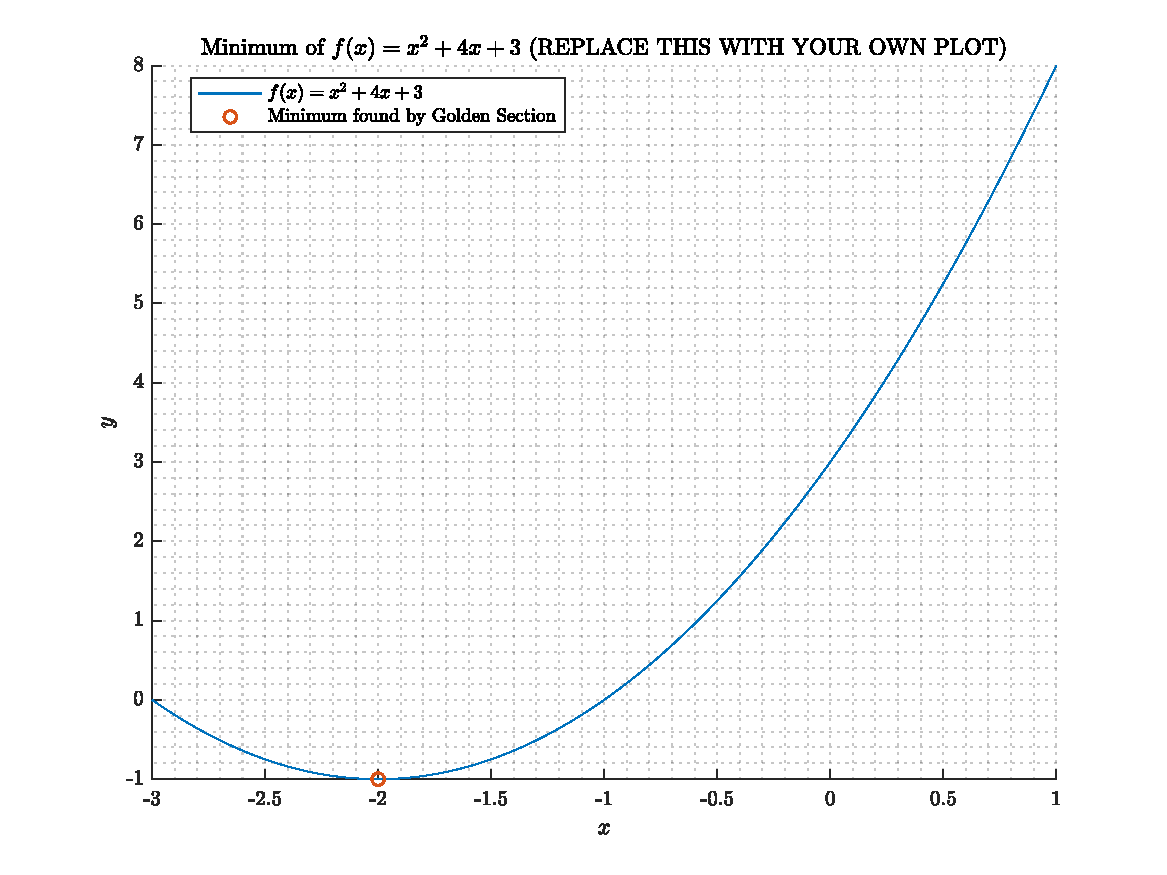
\includegraphics[width=0.8\linewidth]{../src/hw8_p3.pdf}
      \caption{Minimum of $f(x)$ }%
      \label{fig:hw8_p3}
    \end{figure}
  \item Function file \verb|goldenSection.m|:
    \lstinputlisting[style=MATLAB]{../src/goldenSection.m}
  \item Script file \verb|hw8_p3.m|:
    \lstinputlisting[style=MATLAB]{../src/hw8_p3.m}
  \end{itemize}
\end{solution}

